Im Folgenden sollen die beschriebenen Ergebnisse aus den vorherigen Abschnitten \ref{sec:ergebnisseSichtpruefungDurchLichtstreuung} und \ref{sec:ergebnisseDeflektometrischeRegistrierung} aufgegriffen und bewertet werden.
Das Ziel ist es, abhängig vom Anwendungsfall ein passendes Verfahren vorzuschlagen und die Schwächen und Stärken der Verfahren darzulegen.

\p
Für das Verfahren \glqq Sichtprüfung durch Lichtstreuung\grqq ~fällt im Abschnitt \ref{sec:ergebnisseSichtpruefungDurchLichtstreuung} auf, dass es sich besonders gut für die Durchlichtauswertung von transparenten Prüfobjekten eignet.
Es ist möglich bereits sehr kleine Defekte, wie z. B. leichte Kratzer oder Laser-Gravuren auf den Objektoberflächen zu erkennen (siehe Abbildung \ref{tikz:abbErkennbareKleineDefekteLichtstreuung}).

% Abbildung: Erkennbare kleine Defekte
{
	\begin{figure}[H]
		\centering
		\begin{tikzpicture}[every node/.style={inner sep=0,outer sep=0}]

	\node [anchor=north east] (img1) at (-0.03\textwidth,0) {\includegraphics[width=.4\textwidth]{05_ergebnisse/ergDiskussion/figures/lasergravur}};
	\node [below=0.2cm of img1] {Ausschnitt von Brillenglas 1};
	\node [anchor=north west] (img2) at (0.03\textwidth,0) {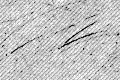
\includegraphics[width=.4\textwidth]{05_ergebnisse/ergDiskussion/figures/polierfehler}};
	\node [below=0.2cm of img2] {Ausschnitt von Brillenglas 2};
	
\end{tikzpicture}
\caption[Erkennbare kleine Defekte oder Laser-Gravur]{Erkennbare kleine Defekte oder Laser-Gravuren durch Durchlichtauswertung mit Verfahren \glqq Sichtprüfung durch Lichtstreuung\grqq ~(siehe Kapitel \ref{chp:sichtpruefungDurchLichtstreuung}) Linkes Teilbild: Erkennbare Lasergravur, Rechtes Teilbild: Leichte Kratzer durch Fehler bei der Polierung}
		\label{tikz:abbErkennbareKleineDefekteLichtstreuung}
	\end{figure}
}

\noindent
Außerdem ist es möglich, für transparente Objekte durch die Durchlichtauswertung auch Defekte im Inneren des Objekts, wie z. B. Lufteinschlüsse in Gläsern, festzustellen.
Dies konnte allerdings nicht nachgeprüft werden, da solche Defekte in den zur Verfügung stehenden Prüfobjekten nicht vorhanden waren.

\p
Für nicht-transparente Prüfobjekte kann das Verfahren \glqq Sichtprüfung durch Lichtstreuung\grqq ~durch eine Spiegelbildauswertung ebenfalls geeignete Bilder erzeugen, um Defekte zu detektieren, allerdings gibt es hierbei schon erste Probleme.
Eine große Schwäche des Verfahrens ist die Abhängigkeit von Oberflächenbeschriftungen oder -aufdrucken.
Da stets Grauwerte der Kamerabilder verknüpft werden, beeinflussen unterschiedliche Farben auf der Oberfläche das Ergebnis (siehe Abbildung \ref{img:delleBeschriftung}).
Das gleiche Phänomen lässt sich auch beobachten, wenn das Objekt abhängig von der Position unterschiedlich stark reflektierend ist.

% Abbildung: Beschriftung Delle
{
	\begin{figure}[H]
		\centering
		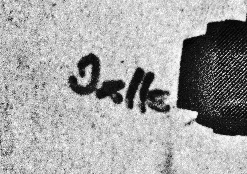
\includegraphics[width=0.4\textwidth]{05_ergebnisse/ergDiskussion/figures/delleBeschriftung}
		\caption[Sichtbare Beschriftung nach Anwendung des Verfahrens aus Kapitel \ref{chp:sichtpruefungDurchLichtstreuung}]{Sichtbare Beschriftung \glqq Delle\grqq ~nach Anwendung des Verfahren \glqq Sichtprüfung durch Lichtstreuung\grqq auf Keramikobjekt 2. Ausschnitt aus Abbildung \ref{tikz:abbNachbearbeitungSpLichtstreuung}}
		\label{img:delleBeschriftung}
	\end{figure}
}

\noindent
Dieser Einfluss kann zu Fehlern in der nachfolgenden Auswertung des Ergebnisbilds durch herkömmliche Bildverarbeitungsalgorithmen führen.
Für dieses Verfahren ist es also notwendig, dass das Prüfobjekt einfarbig und ohne Beschriftungen vorliegt.
Außerdem sollte das Prüfobjekt an allen zu untersuchenden Stellen das Licht gleich stark reflektieren.
Damit können kleinere Defekte, wie z. B. Oberflächenpickel oder Kratzer in Brillengläsern, effizient detektiert werden.
Größere Defekte, wie z. B. die Delle auf der Oberfläche des Keramikobjekts 2 (siehe Abbildung \ref{tikz:abbNachbearbeitungSpLichtstreuung}), sind hingegen schwerer zu identifizieren.
Dieselben Effekte in den Ergebnisbildern wie bei Dellen können auch bei stärker gekrümmten Objekten oder an matten Stellen auftreten.

\p
Die deflektometrische Registrierung erzeugt lediglich die Zuordnungsinformation, die durch spezielle Algorithmen weiterverarbeitet werden muss, um Untersuchungen der Oberfläche zu treffen.
In dem Abschnitt \ref{sec:ergebnisseDeflektometrischeRegistrierung} musste zunächst ein Bild aus der deflektometrischen Registrierung der Zeilen erzeugt werden, damit sich Bildverarbeitungsalgorithmen anwenden lassen.
Die Bildverarbeitung konnte damit bestimmte Auffälligkeiten der Oberflächen hervorheben.
Allerdings verliert man nach dem vorgestellten Ansatz eventuell Informationen über sehr kleine Defekte, da bei der Bilderzeugung je nach verwendeter Farbtiefe\footnote
{
Die Farbtiefe eines Bildes bestimmt die Anzahl differenzierbarer Helligkeitsstufen pro Bildpunkt.
Herkömmlich werden 256 Helligkeitsabstufungen bzw. 8-Bit verwendet.
Mit einer Farbtiefe von 16-Bit hat man bereits 65536 Helligkeitsabstufungen, aber der Speicherbedarf steigt stark an.
%
} mehrere Zeilenpositionen demselben Grauwert zugeordnet werden.
Zur Erzeugung der Ergebnisse in Abschnitt \ref{sec:ergebnisseDeflektometrischeRegistrierung} werden 256 verschiedene Grauwerte unterschieden.
Da aber die Monitorhöhe mehr Positionen als die 256 zu vergebenden Grauwerte hat, fallen verschiedene Zeilen auf denselben Grauwert.
Man verliert Detailinformationen der deflektometrischen Registrierung.
Das macht es schwieriger, sehr kleine Abweichungen der Reflexionen, wie z. B. Kratzer oder Laser-Gravuren, zu erkennen.
Die tatsächlichen Reflexionsabweichungen sind bei der Durchlichtauswertung kleiner als im Spiegelbild.
Es lässt sich auch in Abbildung \ref{tikz:abbAbleitungRegistrierungDurchlicht} erkennen, dass sich die deflektometrische Registrierung für die Durchlichtauswertung von Brillengläsern nur begrenzt eignet.
Auch die Auswertung des Spiegelbilds von Brillenglas 1 zeigt keine Auffälligkeiten, da die Kratzer und Laser-Gravuren die Reflexion des Lichts nur minimal beeinflussen (siehe Abbildung \ref{tikz:abbAbleitungRegistrierungSpiegel}).
Eine mögliche Begründung könnte deshalb die zu geringe Farbtiefe der erzeugten Bilder aus der deflektometrischen Registrierung sein.
Allerdings konnte dies nicht nachgeprüft werden, weshalb die Verbesserung durch eine höhere Farbtiefe in den Ausblick verschoben wird.

\p
Für die Spiegelbildauswertung durch die Bestimmung der deflektometrischen Registrierung der Zeilen sind für die untersuchten Keramikobjekte bessere Ergebnisse zu erkennen (siehe Abbildung \ref{tikz:abbErkennbareDefekteRegistrierung}).

% Abbildung: Erkennbare Defekte
{
	\begin{figure}[H]
		\centering
		\begin{tikzpicture}[every node/.style={inner sep=0,outer sep=0}]

	\node [anchor=north east] (img1) at (-0.03\textwidth,0) {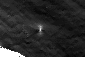
\includegraphics[width=.4\textwidth]{05_ergebnisse/ergDiskussion/figures/pickel}};
	\node [below=0.2cm of img1, align=center] {Ausschnitt von Keramikobjekt 1 \\ aus Abbildung \ref{tikz:abbAbleitungRegistrierungSpiegel}};
	\node [anchor=north west] (img2) at (0.03\textwidth,0) {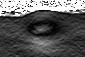
\includegraphics[width=.4\textwidth]{05_ergebnisse/ergDiskussion/figures/delle}};
	\node [below=0.2cm of img2, align=center] {Ausschnitt von Keramikobjekt 2 \\ aus Abbildung \ref{tikz:abbAbleitungRegistrierungSpiegel}};
	
\end{tikzpicture}
\caption[Erkennbare Oberflächendefekte durch deflektometrische Registrierung]{Erkennbare Oberflächendefekte durch Ableitung der deflektometrischen Registrierung. Linkes Teilbild: Oberflächenpickel, Rechtes Teilbild: Delle in der Oberfläche}
		\label{tikz:abbErkennbareDefekteRegistrierung}
	\end{figure}
}

\noindent
Ein großer Vorteil der Auswertung über die deflektometrische Registrierung ist die Unabhängigkeit von Oberflächenbeschriftungen oder -aufdrucken.
Es ist also möglich, ein Objekt mit verschiedenen Farben oder Lackierungen zu prüfen.
Außerdem erhält man durch das Verfahren tatsächliche Krümmungsinformationen der Objektoberfläche, die ausgewertet werden können.
Eine Schwäche der deflektometrischen Registrierung ist die Empfindlichkeit gegenüber Fremdlichteinwirkungen oder störenden Reflexionen, wie z. B. dem Rückseitenreflex bei spiegelnden Oberflächen (siehe Abbildung \ref{tikz:abbRückseitenreflexRegistrierung}).

% Abbildung: Rückseitenreflex Registrierung
{
	\begin{figure}[H]
		\centering
		\input{05_ergebnisse/ergDiskussion/figures/abbRückseitenreflexRegistrierung}
		\label{tikz:abbRückseitenreflexRegistrierung}
	\end{figure}
}

\noindent
Durch die Überlagerung der Reflexionen im Kamerabild ist es nicht länger möglich, die Dekodierung korrekt durchzuführen.
Es kommt an manchen Stellen zu Fehlern und Phasensprüngen.
Dadurch wird auch die Auswertung des Bildes keine nützlichen Ergebnisse mehr erbringen können.

\p
Die Problematik des Rückseitenreflexes trifft auch auf das Verfahren \glqq Sichtprüfung durch Lichtstreuung\grqq ~zu.
Durch die überlagerten Streifenmuster kann es passieren, dass fehlerhafte Strukturen durch das Verfahren entstehen (siehe Abbildung \ref{tikz:abbRückseitenreflexLichtstreuung}).

% Abbildung: Rückseitenreflex Lichtstreuung
{
	\begin{figure}[H]
		\centering
		\input{05_ergebnisse/ergDiskussion/figures/abbRückseitenreflexLichtstreuung}
		\label{tikz:abbRückseitenreflexLichtstreuung}
	\end{figure}
}

\noindent
Durch die bisherigen Ausführungen lassen sich in den vorgestellten Verfahren Stärken und Schwächen erkennen.
Ausgehend davon soll die Eignung der Verfahren für spezielle Anwendungen vermittelt werden.
Aus Abbildungen \ref{tikz:abbRückseitenreflexRegistrierung} und \ref{tikz:abbRückseitenreflexLichtstreuung} lässt sich schließen, dass transparente Objekte durch den Rückseitenreflex nicht für die Spiegelbildauswertung mit den vorgestellten Verfahren geeignet sind.
Aufgrund der hohen Empfindlichkeit bei der Durchlichtauswertung bietet sich deshalb besonders das Verfahren \glqq Sichtprüfung durch Lichtstreuung\grqq ~an, wenn die qualitative Sichtprüfung des transparenten Objekts ausreichend ist.
Sobald weitere Informationen, wie z. B. die Oberflächenkrümmung erforderlich sind, sollte für die Objekte die deflektometrische Registrierung des Spiegelbilds bestimmt werden.
Dabei muss dann auch das Problem des Rückseitenreflexes behandelt werden.

\p
Es wird ersichtlich, dass das Verfahren zur Auswertung der deflektometrischen Registrierung bessere Ergebnisse für nicht-transparente spiegelnde Objekte bei der Spiegelbildanalyse erzielen kann.
Im Vergleich zum Verfahren \glqq Sichtprüfung durch Lichtstreuung\grqq ~ist die deflektometrische Registrierung besser geeignet für stärker gekrümmte oder lackierte Objekte.
Die deflektometrische Registrierung kann durch weitere Verarbeitungen auch genutzt werden, um die Oberfläche des Prüfobjekts zu rekonstruieren.
Diese Möglichkeiten machen die deflektometrische Registrierung zu einer nützlichen Information über Oberflächen zur Erfassung von Oberflächendefekten spiegelnder Objekte.